%\chapter*{Introdução}
%\begin{center}
  \vspace{1.2em}
  \textbf{\large INTRODUÇÃO}
  \vspace{2.9em}
%\end{center}
\thispagestyle{empty}

\addcontentsline{toc}{chapter}{INTRODUÇÃO}
\stepcounter{chapter} %incrementa o número do capítulo

	\par Atualmente, com os avanços tecnológicos, as pessoas estão cada vez mais
conectadas e procuram soluções para seus problemas, que possam ajudá-las de
forma rápida e fácil.  Segundo \citeonline{lacheta2013}, tanto as empresas
quantos os desenvolvedores buscam plataformas modernas e ágeis para a criação
de aplicações. Esse fato contribuiu consideravelmente para o crescimento das
plataformas móveis de comunicação.

	\par Uma das áreas que mais se expandiu nos últimos anos é a de telefonia
móvel. \citeonline[p.1]{monteiro2012} afirma que “os telefones celulares foram
evoluindo, ganhando cada vez mais recursos e se tornando um item quase
indispensável na vida das pessoas”. Essa evolução no hardware possibilitou o
crescimento, mobilidade e portabilidade do software.

	\par Muitas coisas que antes eram feitas apenas em computadores
\textit{desktops} já podem ser realizadas nos celulares, como transferências
bancárias, localização de taxi, conversas entre amigos, entretenimento com
jogos e vídeos, entre outros. Ainda de acordo com \citeonline{monteiro2012}, a
plataforma Android se destaca no mercado devido ao grande número de aparelhos
espalhados pelo mundo além das facilidades que provêem aos desenvolvedores. Na
Figura \ref{fig:intro}, é possível ver um gráfico informando que no ano de
2016, 52,9\% dos \textit{smartphones} terão o sistema operacional Android.

	\begin{figure}[h!]
		\centerline{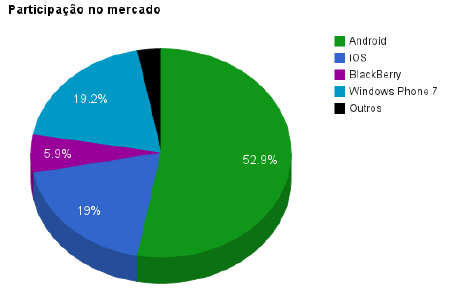
\includegraphics[scale=1]{./imagens/0_introducao/introducao.png}}
		\caption[Participação de mercado do Android em 2016]{Participação de
		mercado do Android em 2016.
		\textbf{Fonte:}\citeonline{monteiro2012}}
		\label{fig:intro}
	\end{figure}

	\par Hoje em dia, há uma gama enorme de aplicativos para Android que tem como
objetivo resolver problemas específicos. \citeonline{mendes2011}, vendo as
dificuldades encontradas pelas novas bandas musicais em saber as opiniões de
seus fãs referente a \textit{shows} realizados, criou um aplicativo que tornou
possível a interação entre eles. \citeonline{oglio2013}, desenvolveu um
utilitário para Android que possibilitou aos alunos do Centro Universitário
Univates acessarem o portal virtual de sua faculdade.


	\par Pensando-se nas facilidades providas pelos dispositivos móveis em
conseguir informações rápidamente, a qualquer hora e local e visando facilitar
o acesso dos alunos as suas notas, faltas e provas agendadas, esta pesquisa tem
por objetivos desenvolvolver um aplicativo para a plataforma Android que
possibilite aos alunos da Universidade do Vale do Sapucaí receberem
notificações e consultarem suas notas, faltas e provas agendadas do semestre
corrente, bem como deselvolver um \textit{web service} que provê uma estrutura
para a Univás disponibilizar seus dados através de serviço.

%\chapter{OBJETIVOS}
	
	\par Para alcançar o propósito principal do trabalho, o objetivo geral foi
dividido em alguns objetivos específicos, aos quais pode-se citar:
	
	\begin{itemize}
	  
	  \item Levantar requisitos do software proposto de acordo com as
	  necessidades dos discentes.
	  
	  \item Desenvolver um aplicativo para dispositivos móveis na plataforma
	  Android.
	  
	  \item Desenvolver um \textit{web service} que possibilitará a Univás
	  disponibilizar suas informações através de serviços e implemetar um serviço
	  para que o aplicativo Android consulte as informações  relativas a notas,
	  faltas e provas agendadas.
	
	\end{itemize}
	
	\par Desta maneira, esse trabalho contribui socialmente com os graduandos, pois
espera-se agilizar o processo em que eles consultam os resultados dos
exercícios avaliativos, faltas e as provas agendadas. O software também irá
notificá-los no momento em que houver algum lançamento referente às disciplinas
cursadas, evitando assim que o estudante tenha que acessar o portal do aluno
várias vezes ao dia, ansioso em saber seu rendimento.

	\par O projeto coopera na qualificação dos envolvidos do trabalho, tendo em
vista o aumento na procura por profissionais habilitados com tecnologias atuais
como Java, Android, REST\footnote{REST - \textit{Representational State
Transfer} ou Transferência de Estado Representativo.}, Hibernate entre outros.

	\par Para a universidade, essa pesquisa a coloca como pioneira neste quesito e
demostra a sua preocupação com o bem estar de seus alunos, pois existem pessoas
que não tem computadores, mas possuem \textit{smartphones}, com isso eles
também conseguirão ter suas informações. O \textit{web service} coloca ao
alcançe da Univás a estrutura para disponibilizar seus dados através de
serviço.

	\par Na área acadêmica, esse trabalho contribui aos alunos do curso de Sistemas
de Informação servindo lhes como referência para pesquisas futuras ou usá-lo
para adicionar funcionalidades a este projeto.

	\par Este trabalho é composto de quatro capítulos, sendo que o atual faz uma
breve introdução sobre o tema proposto e seus objetivos. No segundo capítulo é
descrito as teorias sobre as tecnologias utilizadas para o desenvolvimento do
projeto. O terceiro, relata as metodologias usadas nesta pesquisa, bem como,
tipo de pesquisa, contexto de pesquisa, instrumentos e procedimentos. No quarto
capítulo é realizado a discussão de resultados ressaltando o que se obteve com
a realização do trabalho. Por fim, é realizado a conclusão.
